\documentclass[xcolor=table]{beamer}

\usepackage[T1]{fontenc}
\usepackage[utf8]{inputenc}
\usepackage{lmodern}
\usepackage{tikz}
\usetikzlibrary{positioning,calc}
\usepackage{tcolorbox}
\usepackage{booktabs}
\usepackage{colortbl}
\usepackage{fontawesome5}
\usepackage{enumitem}

% ---------- palette ----------
\definecolor{corpnavy}{RGB}{20,34,64}
\definecolor{corpnavylight}{RGB}{38,56,92}
\definecolor{corpteal}{RGB}{15,139,141}
\definecolor{corpgold}{RGB}{201,162,39}
\definecolor{corpgray}{RGB}{237,239,241}
\definecolor{corptext}{RGB}{45,52,63}

% ---------- beamer setup ----------
\usetheme{default}
\usefonttheme{professionalfonts}
\setbeamertemplate{navigation symbols}{}
\setbeamercolor{background canvas}{bg=white}
\setbeamercolor{normal text}{fg=corptext}
\setbeamercolor{structure}{fg=corpnavy}
\setbeamercolor{frametitle}{fg=corpnavy,bg=white}
\setbeamercolor{footline}{fg=corpnavy!55!white,bg=corpgray}
\setbeamercolor{itemize item}{fg=corpteal}
\setbeamercolor{itemize subitem}{fg=corpgold}
\setbeamerfont{frametitle}{series=\bfseries,size=\Large}
\setbeamerfont{footline}{size=\scriptsize}
\setbeamertemplate{itemize item}{\faArrowRight}
\setbeamertemplate{itemize subitem}{\textbullet}

\setbeamertemplate{frametitle}{%
  \nointerlineskip
  \begin{beamercolorbox}[wd=\paperwidth,sep=0.35cm,leftskip=0.5cm]{frametitle}
    \usebeamerfont{frametitle}\insertframetitle\par
    \vspace{2pt}{\color{corpgold}\rule{2.6cm}{1.4pt}}
  \end{beamercolorbox}
}

\setbeamertemplate{footline}{%
  \leavevmode
  \hbox{\begin{beamercolorbox}[wd=\paperwidth,ht=2.6ex,dp=1.2ex,leftskip=0.5cm,rightskip=0.5cm]{footline}
    \usebeamerfont{footline}NEXA \textbar\ Quarterly Business Review \hfill Q3 FY2026 \hfill \insertframenumber{}/\inserttotalframenumber
  \end{beamercolorbox}}
}

\newtcolorbox{kpibox}{%
  colback=white,colframe=corpteal!65!black,boxrule=0.5pt,arc=2pt,
  left=7pt,right=7pt,top=7pt,bottom=6pt,boxsep=0pt
}

\newtcolorbox{calloutbox}[1][corpteal]{%
  colback=corpgray,colframe=#1!70!black,boxrule=0.6pt,arc=2pt,
  left=9pt,right=9pt,top=7pt,bottom=7pt
}

\newcommand{\sectiondivider}[3]{%
{%
\setbeamertemplate{footline}{}
\begin{frame}[plain]
\begin{tikzpicture}[remember picture,overlay]
\fill[corpnavy] (current page.south west) rectangle (current page.north east);
\draw[corpteal!60!white,line width=0.6pt] ([yshift=1.7cm]current page.south west) -- ([yshift=1.7cm]current page.south east);
\node[align=center,text=white] at ([yshift=0.3cm]current page.center) {%
  {\color{corpgold}\bfseries\fontsize{13}{15}\selectfont #1}\\[10pt]
  {\bfseries\fontsize{30}{34}\selectfont #2}\\[8pt]
  {\itshape\color{corpteal!35!white}\fontsize{13}{15}\selectfont #3}%
};
\node[anchor=south west,text=corpteal!50!white,font=\scriptsize] at ([xshift=0.6cm,yshift=0.5cm]current page.south west) {NEXA \textbar\ Quarterly Business Review \textbar\ Q3 FY2026};
\end{tikzpicture}
\end{frame}
}}

\title{Quarterly Business Review}
\author{Nexa}
\date{}

\begin{document}

% ---------------- Title slide ----------------
{%
\setbeamertemplate{footline}{}
\begin{frame}[plain]

\begin{tikzpicture}[remember picture,overlay]
\fill[corpnavy] (current page.south west) rectangle (current page.north east);
\fill[corpgold] ([yshift=2.0cm]current page.south west) rectangle ([yshift=2.08cm]current page.south east);
\node[anchor=west,text=corpgold,font=\bfseries\fontsize{15}{17}\selectfont] at ([xshift=1.1cm,yshift=5.4cm]current page.south west) {NEXA};
\node[anchor=west,text=white,font=\bfseries\fontsize{30}{34}\selectfont,align=left] at ([xshift=1.1cm,yshift=4.35cm]current page.south west) {Quarterly Business Review};
\node[anchor=west,text=corpteal!45!white,font=\itshape\fontsize{15}{18}\selectfont] at ([xshift=1.1cm,yshift=3.6cm]current page.south west) {Q3 FY2026 \textbar\ Period Ended September 30, 2026};
\node[anchor=west,text=white,font=\bfseries\fontsize{12}{14}\selectfont] at ([xshift=1.1cm,yshift=2.7cm]current page.south west) {Elena Marsh};
\node[anchor=west,text=corpteal!45!white,font=\fontsize{10}{12}\selectfont] at ([xshift=1.1cm,yshift=2.35cm]current page.south west) {SVP, Strategy \& Operations \textbar\ Nexa};
\node[anchor=west,text=corpteal!35!white,font=\scriptsize] at ([xshift=1.1cm,yshift=1.0cm]current page.south west) {Prepared for the Board of Directors \textbar\ Confidential -- Internal Use Only};
\node[anchor=east,text=corpteal!35!white,font=\scriptsize] at ([xshift=-1.1cm,yshift=1.0cm]current page.south east) {October 14, 2026};
\end{tikzpicture}
\end{frame}
}

% ---------------- Agenda ----------------
\begin{frame}{Agenda}
\begin{columns}[T]
\begin{column}{0.06\textwidth}
\end{column}
\begin{column}{0.88\textwidth}
\begin{enumerate}[label=\textbf{\textcolor{corpteal}{0\arabic*}},leftmargin=1.1cm,itemsep=8pt]
\item \textbf{Executive Summary} --- {\small\itshape headline KPIs}
\item \textbf{Financial Performance} --- {\small\itshape revenue by segment \& trend}
\item \textbf{Operational Highlights} --- {\small\itshape delivery \& roadmap}
\item \textbf{Market \& Competitive Landscape} --- {\small\itshape positioning \& wins}
\item \textbf{Outlook \& Risks} --- {\small\itshape Q4 guidance}
\end{enumerate}
\vspace{8pt}
\begin{calloutbox}[corpgold]
\small\faCalendar\ \ \textbf{Today's goal:} align the Board on Q3 results, confirm Q4 guidance,
and flag the two risks that most affect the FY2026 exit rate.
\end{calloutbox}
\end{column}
\begin{column}{0.06\textwidth}
\end{column}
\end{columns}
\end{frame}

% ---------------- Section divider 1 ----------------
\sectiondivider{SECTION 01}{Executive Summary}{Headline results and the quarter in one page}

% ---------------- KPI scorecard ----------------
\begin{frame}{Q3 FY2026 KPI Scorecard}
\begin{minipage}[t]{0.235\textwidth}
\begin{kpibox}
\centering{\color{corpteal}\Large\faChartLine}\par
\vspace{3pt}{\color{corpnavy}\bfseries\Large \$48.2M}\par
{\small Total Revenue}\par
{\scriptsize\color{corpteal!60!black} +18\% YoY}
\end{kpibox}
\end{minipage}\hfill
\begin{minipage}[t]{0.235\textwidth}
\begin{kpibox}
\centering{\color{corpteal}\Large\faRocket}\par
\vspace{3pt}{\color{corpnavy}\bfseries\Large \$186.4M}\par
{\small Annual Recurring Revenue}\par
{\scriptsize\color{corpteal!60!black} +22\% YoY}
\end{kpibox}
\end{minipage}\hfill
\begin{minipage}[t]{0.235\textwidth}
\begin{kpibox}
\centering{\color{corpteal}\Large\faHandshake}\par
\vspace{3pt}{\color{corpnavy}\bfseries\Large 114\%}\par
{\small Net Revenue Retention}\par
{\scriptsize\color{corpteal!60!black} +3 pts QoQ}
\end{kpibox}
\end{minipage}\hfill
\begin{minipage}[t]{0.235\textwidth}
\begin{kpibox}
\centering{\color{corpteal}\Large\faUsers}\par
\vspace{3pt}{\color{corpnavy}\bfseries\Large 2{,}340}\par
{\small Active Customers}\par
{\scriptsize\color{corpteal!60!black} +9\% QoQ}
\end{kpibox}
\end{minipage}
\par
\vspace{9pt}
\small\textbf{\color{corpnavy}Reading the quarter:} growth accelerated on the back of the
Nexa Insights 3.0 launch and a strong renewal cycle in the enterprise segment. Retention
crossed 110\% for the second consecutive quarter, and the customer base grew past 2{,}300
accounts for the first time.
\begin{itemize}[itemsep=3pt]
\small
\item Enterprise tier now represents 61\% of ARR, up from 54\% a year ago
\item Gross margin held at 78.4\%, in line with FY2026 guidance
\item Two logo losses in the SMB tier, attributed to budget consolidation, not product fit
\end{itemize}
\end{frame}

% ---------------- Section divider 2 ----------------
\sectiondivider{SECTION 02}{Financial Performance}{Revenue by segment and the quarterly trend line}

% ---------------- Revenue table ----------------
\begin{frame}{Revenue by Segment}
\renewcommand{\arraystretch}{1.25}
\begin{center}
\begin{tabular}{lrrr}
\toprule
\rowcolor{corpnavy}
{\color{white}\textbf{Segment}} & {\color{white}\textbf{Q3 FY25}} & {\color{white}\textbf{Q3 FY26}} & {\color{white}\textbf{YoY}} \\
\midrule
Core Platform Subscriptions & \$24.1M & \$28.6M & \textcolor{corpteal!70!black}{+18.7\%} \\
Analytics \& Insights Add-ons & \$6.8M & \$9.4M & \textcolor{corpteal!70!black}{+38.2\%} \\
Professional Services & \$4.9M & \$5.7M & \textcolor{corpteal!70!black}{+16.3\%} \\
International (EMEA/APAC) & \$4.9M & \$4.5M & \textcolor{red!60!black}{-8.2\%} \\
\midrule
\rowcolor{corpgray}
\textbf{Total Revenue} & \textbf{\$40.7M} & \textbf{\$48.2M} & \textbf{\textcolor{corpteal!70!black}{+18.4\%}} \\
\bottomrule
\end{tabular}
\end{center}
\vspace{12pt}
\begin{calloutbox}
\faExclamationTriangle\ \ \textbf{Watch item:} International revenue declined for the second
straight quarter on FX translation and a slower APAC renewal cycle; underlying bookings in
constant currency were flat.
\end{calloutbox}
\end{frame}

% ---------------- Revenue trend chart ----------------
\begin{frame}{Quarterly Revenue Trend}
\begin{center}
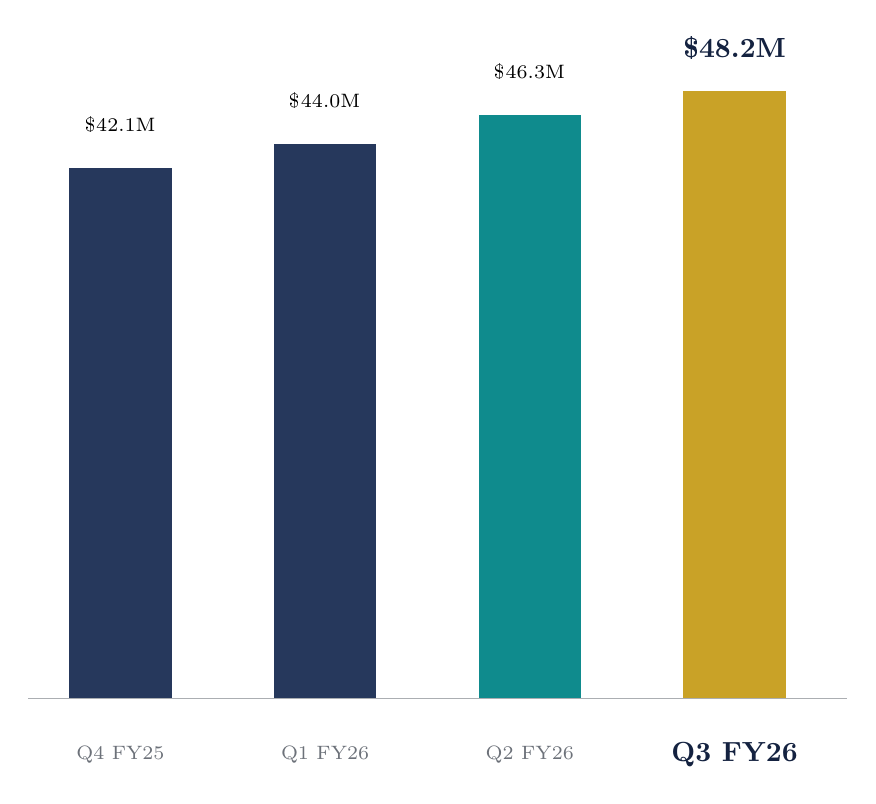
\begin{tikzpicture}[x=2.6cm,y=0.16cm]
\draw[corptext!40!white] (0.3,0) -- (4.3,0);
% Q4 FY25
\fill[corpnavylight] (0.5,0) rectangle (1.0,42.1);
\node[font=\scriptsize] at (0.75,45.5) {\$42.1M};
\node[font=\scriptsize,text=corptext!70!white] at (0.75,-4.5) {Q4 FY25};
% Q1 FY26
\fill[corpnavylight] (1.5,0) rectangle (2.0,44.0);
\node[font=\scriptsize] at (1.75,47.4) {\$44.0M};
\node[font=\scriptsize,text=corptext!70!white] at (1.75,-4.5) {Q1 FY26};
% Q2 FY26
\fill[corpteal] (2.5,0) rectangle (3.0,46.3);
\node[font=\scriptsize] at (2.75,49.7) {\$46.3M};
\node[font=\scriptsize,text=corptext!70!white] at (2.75,-4.5) {Q2 FY26};
% Q3 FY26
\fill[corpgold] (3.5,0) rectangle (4.0,48.2);
\node[font=\scriptsize,text=corpnavy,font=\bfseries] at (3.75,51.6) {\$48.2M};
\node[font=\scriptsize,text=corpnavy,font=\bfseries] at (3.75,-4.5) {Q3 FY26};
\end{tikzpicture}
\end{center}
\vspace{10pt}
\begin{center}
\begin{minipage}{0.85\textwidth}
\centering\small
Five consecutive quarters of sequential growth, averaging \textbf{+4.6\% QoQ}.
The Q3 step-up coincides with the general availability of Nexa Insights 3.0 in August.
\end{minipage}
\end{center}
\end{frame}

% ---------------- Section divider 3 ----------------
\sectiondivider{SECTION 03}{Operational Highlights}{Delivery, customer success, and what ships next}

% ---------------- Operational highlights bullets ----------------
\begin{frame}{Operational Highlights}
\begin{columns}[T]
\begin{column}{0.48\textwidth}
\textbf{\color{corpnavy}\faCogs\ \ Product \& Engineering}
\begin{itemize}[itemsep=6pt]
\item Nexa Insights 3.0 shipped on schedule, adding real-time cohort analysis
\item Platform uptime held at 99.97\%, above the 99.9\% SLA target
\item Reduced median query latency by 31\% following the storage-layer migration
\end{itemize}
\vspace{8pt}
\textbf{\color{corpnavy}\faComments\ \ Customer Success}
\begin{itemize}[itemsep=6pt]
\item Onboarding time-to-value cut from 19 to 12 days for enterprise accounts
\item Launched quarterly business reviews for all Nexa Enterprise customers
\end{itemize}
\end{column}
\begin{column}{0.48\textwidth}
\textbf{\color{corpnavy}\faUsers\ \ People}
\begin{itemize}[itemsep=6pt]
\item Headcount reached 412, with 28 net new hires in Q3
\item Opened a Singapore hub to support APAC delivery and support coverage
\end{itemize}
\vspace{8pt}
\begin{calloutbox}[corpgold]
\faTrophy\ \ \textbf{Milestone:} Nexa passed 2{,}300 active customers and crossed
\$180M in ARR for the first time this quarter.
\end{calloutbox}
\end{column}
\end{columns}
\end{frame}

% ---------------- Roadmap timeline ----------------
\begin{frame}{Q4 FY2026 Roadmap}
\begin{center}
\resizebox{\linewidth}{!}{%

\begin{tikzpicture}[
  node distance=0.9cm and 1.55cm,
  every node/.style={font=\small},
  milestone/.style={rectangle,rounded corners=3pt,draw=corpteal!70!black,
    fill=corpgray,text width=2.5cm,align=center,minimum height=1.3cm,inner sep=4pt}
]
\node[milestone] (m1) {Nexa Insights 3.0 GA \\[2pt] {\scriptsize\color{corpteal!70!black} October}};
\node[milestone,right=of m1,fill=corpteal,text=white] (m2) {EMEA Data Residency GA \\[2pt] {\scriptsize\color{white} November}};
\node[milestone,right=of m2] (m3) {Enterprise SSO \& Audit Log GA \\[2pt] {\scriptsize\color{corpteal!70!black} December}};
\node[milestone,right=of m3,fill=corpnavy,text=white] (m4) {Nimbus Partnership Kickoff \\[2pt] {\scriptsize\color{corpgold} January}};
\draw[->,thick,corpteal!60!black] (m1) -- (m2);
\draw[->,thick,corpteal!60!black] (m2) -- (m3);
\draw[->,thick,corpteal!60!black] (m3) -- (m4);
\end{tikzpicture}
}%
\end{center}
\vspace{14pt}
\centering\small
Each milestone has an assigned executive sponsor and a Go/No-Go review two weeks prior to launch.
\end{frame}

% ---------------- Section divider 4 ----------------
\sectiondivider{SECTION 04}{Market \& Competitive Landscape}{Where Nexa is winning, and against whom}

% ---------------- Market slide ----------------
\begin{frame}{Market \& Competitive Landscape}
\begin{itemize}[itemsep=9pt]
\item \faGlobe\ \ The analytics platform market continues to consolidate around three
  vendors: Nexa, Apex Software, and Meridian Data Corp
\item \faTrophy\ \ \textbf{Vertex Retail Group} selected Nexa over Apex Software for its
  enterprise analytics rollout, citing faster time-to-value and stronger implementation support
\item \faHandshake\ \ Announced a data-pipeline integration partnership with
  \textbf{Synapse Systems}, opening a co-sell channel into their installed base
\item \faExclamationTriangle\ \ Meridian Data Corp cut list pricing 12\% in EMEA; two renewal
  negotiations this quarter cited it directly
\end{itemize}
\vspace{10pt}
\begin{calloutbox}
\faBullseye\ \ \textbf{Positioning:} Nexa continues to win on implementation speed and
support quality rather than price -- a durable advantage as long as onboarding time-to-value
keeps improving.
\end{calloutbox}
\end{frame}

% ---------------- Section divider 5 ----------------
\sectiondivider{SECTION 05}{Outlook \& Risks}{Q4 guidance and what could move it}

% ---------------- Outlook & risks ----------------
\begin{frame}{Q4 Guidance \& Key Risks}
\begin{columns}[T]
\begin{column}{0.48\textwidth}
\begin{calloutbox}[corpteal]
\textbf{\color{corpnavy}Q4 FY2026 Guidance}
\begin{itemize}[itemsep=6pt,leftmargin=14pt]
\item Revenue: \$50M -- \$52M
\item FY2026 ARR growth: 20\% -- 24\%
\item Gross margin: 78\% -- 79\%
\end{itemize}
\end{calloutbox}
\end{column}
\begin{column}{0.48\textwidth}
\begin{calloutbox}[corpgold]
\textbf{\color{corpnavy}Top Risks}
\begin{itemize}[itemsep=6pt,leftmargin=14pt]
\item FX headwinds continuing to pressure APAC revenue
\item Key-person dependency in Professional Services delivery
\item Pricing pressure from Meridian Data Corp in EMEA renewals
\end{itemize}
\end{calloutbox}
\end{column}
\end{columns}
\vspace{14pt}
\centering\small
None of the above risks are currently reflected as downside case in guidance; they are
tracked weekly by the Strategy \& Operations team.
\end{frame}

% ---------------- Closing slide ----------------
{%
\setbeamertemplate{footline}{}
\begin{frame}[plain]
\begin{tikzpicture}[remember picture,overlay]
\fill[corpnavy] (current page.south west) rectangle (current page.north east);
\node[align=center,text=white] at ([yshift=0.6cm]current page.center) {%
  {\bfseries\fontsize{26}{30}\selectfont Thank You}\\[10pt]
  {\itshape\color{corpteal!40!white}\fontsize{13}{15}\selectfont Questions \& Board discussion}%
};
\node[align=center,text=corpteal!45!white,font=\small] at ([yshift=-1.6cm]current page.center)
  {\faEnvelope\ \ elena.marsh@nexa-corp.example \quad\quad \faPhone\ \ +1 (415) 555-0148};
\node[anchor=south,text=corpgold,font=\scriptsize] at ([yshift=0.6cm]current page.south)
  {NEXA \textbar\ Confidential -- Internal Use Only};
\end{tikzpicture}
\end{frame}
}

\end{document}
